%%% GRASP, a=0.8, obj= 5min, 5 iterations, 
% Profit = 146
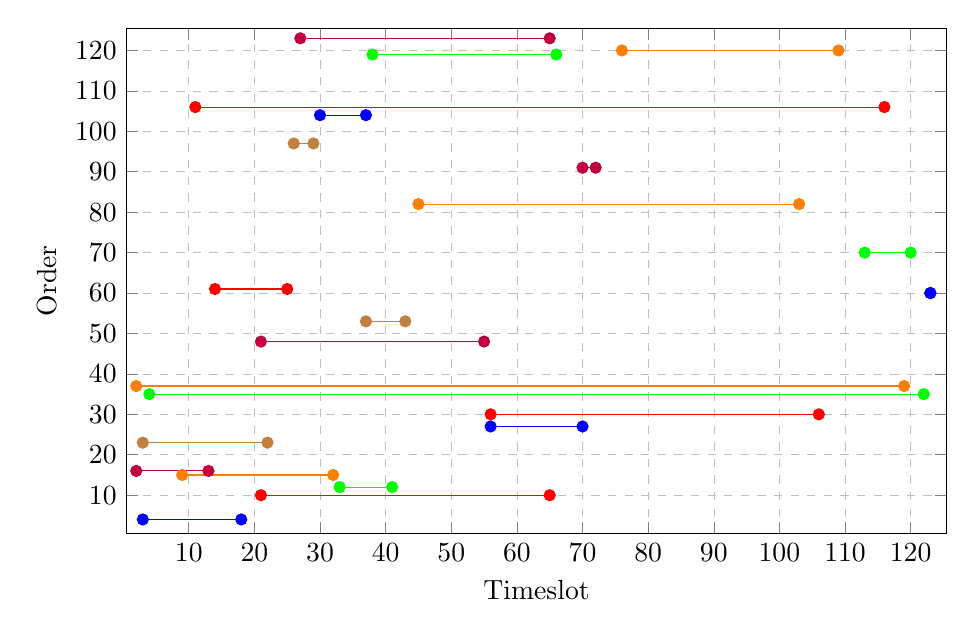
\begin{tikzpicture}
\begin{axis}[
    xlabel={Timeslot},
    ylabel={Order},
    xmin=0.5, xmax=125.5, 
    ymin=0.5, ymax=125.5, 
    xtick={10,20,30,40,50,60,70,80,90,100, 110, 120},
    ytick={10,20,30,40,50,60,70,80,90,100, 110, 120},
    grid=both,
    grid style={line width=.1pt, draw=gray!10},
    major grid style={line width=.2pt, draw=gray!50},
    legend pos=north east,
    ymajorgrids=true,
    xmajorgrids=true,
    grid style=dashed,
     width=12cm,
     height=8cm,
]
\addplot[color=blue, mark=*] coordinates {(3, 4) (18, 4)};
\addplot[color=red, mark=*] coordinates {(21, 10) (65, 10)};
\addplot[color=green, mark=*] coordinates {(33, 12) (41, 12)};
\addplot[color=orange, mark=*] coordinates {(9, 15) (32, 15)};
\addplot[color=purple, mark=*] coordinates {(2, 16) (13, 16)};
\addplot[color=brown, mark=*] coordinates {(3, 23) (22, 23)};
\addplot[color=blue, mark=*] coordinates {(56, 27) (70, 27)};
\addplot[color=red, mark=*] coordinates {(56, 30) (106, 30)};
\addplot[color=green, mark=*] coordinates {(4, 35) (122, 35)};
\addplot[color=orange, mark=*] coordinates {(2, 37) (119, 37)};
\addplot[color=purple, mark=*] coordinates {(21, 48) (55, 48)};
\addplot[color=brown, mark=*] coordinates {(37, 53) (43, 53)};
\addplot[color=blue, mark=*] coordinates {(123, 60) (123, 60)};
\addplot[color=red, mark=*] coordinates {(14, 61) (25, 61)};
\addplot[color=green, mark=*] coordinates {(113, 70) (120, 70)};
\addplot[color=orange, mark=*] coordinates {(45, 82) (103, 82)};
\addplot[color=purple, mark=*] coordinates {(70, 91) (72, 91)};
\addplot[color=brown, mark=*] coordinates {(26, 97) (29, 97)};
\addplot[color=blue, mark=*] coordinates {(30, 104) (37, 104)};
\addplot[color=red, mark=*] coordinates {(11, 106) (116, 106)};
\addplot[color=green, mark=*] coordinates {(38, 119) (66, 119)};
\addplot[color=orange, mark=*] coordinates {(76, 120) (109, 120)};
\addplot[color=purple, mark=*] coordinates {(27, 123) (65, 123)};
\end{axis}
\end{tikzpicture}